\section{Motivation}
\label{sec:motiv}

\subsection{PIM--Host Crossover}
\label{sec:bg:roofline}

% P:mot-roofline-setup
Fig.~\ref{fig:roofline} plots skinny-GEMM throughput against $M$ in the roofline form~\cite{roofline} for the host
NPU's roof and for simulated PIM GEMMs of stock AiM and each platform's rival. Each PIM curve is the geometric mean over
the FC shapes of the platform's models, and Fig.~\ref{fig:roofline} and the later throughput figures plot $M = 2^k$.
The mobile NPU is the Snapdragon 8 Gen 3's~\cite{sd8g3}, which reaches 56\,GB/s~\cite{powerinfer2} of its own
68\,GB/s pins~\cite{heterollm}; applied to the 51.2\,GB/s pins of x64 LPDDR5-6400, that fraction gives the NPU
42\,GB/s\ASSUMPTION. The edge-server NPU is P3-LLM's~\cite{p3llm}. Throughput numbers in this section are modelled on
the mobile platform and the edge server of Table~\ref{tab:params}, which Section~\ref{sec:method} details.

% P:mot-host-roof
\paragraph{Host roof in the skinny range}
The host stays memory-bound across the whole skinny range. The Snapdragon 8 Gen 3 NPU reaches its compute
roof only at $M \approx 143$, and P3-LLM's~\cite{p3llm} NPU reaches its roof at $M = 128$ (Fig.~\ref{fig:roofline}a,
b). Each NPU's ridge lies far above $M = 32$, so the host's roof rises linearly with $M$ across the skinny
range.

% P:mot-stock-crossover
\paragraph{Stock-PIM crossover}
Stock PIM beats the host only for the first few token rows. At $M = 1$ every PIM ceiling starts 9.75$\times$ above the
mobile NPU's roof and 4$\times$ above the edge-server NPU's roof. Stock AiM's ceiling is flat from $M = 1$, however,
because stock AiM repeats the GEMV once per token row, so its GEMM time grows in proportion to $M$. The rising host roof overtakes that ceiling, and stock
AiM wins a whole decode step only up to $M = 6$ on the mobile platform and $M = 2$--3 on the edge server, below most of
the published values of $M$ (Section~\ref{sec:bg:skinny}).

% P:mot-gemv-only
\paragraph{GEMV-only use of PIM}
Stock PIM is a GEMV engine, and published systems keep PIM for GEMVs and send the GEMMs to the host, even though the
host runs every skinny GEMM on its memory roof. AttAcc~\cite{attacc} runs batched FC layers on the xPU and attention on
PIM. NeuPIMs~\cite{neupims} maps the GEMMs to the NPU because PIM ``lacks the computational power to handle GEMM
effectively.'' IANUS~\cite{ianus} chooses NPU or PIM per FC layer. P3-LLM~\cite{p3llm} offloads its linear layers to
the NPU from batch 8, where its PIM becomes compute-bound.

% P:mot-a-summary
Skinny GEMMs are memory-bound on the host and thus belong on PIM, which reads the weights inside the DRAM, yet stock
PIM's GEMM throughput stays flat at its GEMV ceiling. Section~\ref{sec:bg:cmd} splits a stock GEMM's time to locate the
cause.

\subsection{Two Root Causes of Stock PIM Inefficiency}
\label{sec:bg:cmd}

% P:mot-breakdown-setup
Fig.~\ref{fig:breakdown} splits stock AiM's GEMM time into six components for one tile and for the query projection
layer (q\_proj) of Llama-2-7B on the mobile platform and of Llama-3.1-8B on the edge server; each bar is normalised to
its GEMM time, which is printed at the bar's end. The one tile's weights fill one row sweep in each bank and its inputs
fill one GB chunk ($K \times N$ of $2048 \times 64$ on the mobile platform and $4096 \times 256$ on the edge server),
so the one tile shows the costs of one row sweep. The q\_proj kernel, attention's $4096 \times 4096$ query projection,
shows a whole layer. Both kernels run at $M = 8$ on one channel. The mobile platform places an INT8 PU beside each
LPDDR5-6400 bank, and the edge server places a W4A8 PU beside each pair of HBM2 banks (Table~\ref{tab:params}). Each
platform computes at the precision of the prior PIM design that targets it, LP-Spec~\cite{lpspec} on the mobile platform
and P3-LLM~\cite{p3llm} on the edge server. The six
components form two groups: the time in non-MAC commands (row switch, token load, token drain and refresh) and the
time in MAC slots, which hold useful and idle beats. A MAC slot is the time \tslot that one all-bank MAC command
occupies; on the mobile platform a MAC slot spans one column period (Fig.~\ref{fig:dram_pim}b). Useful MAC work fills
at most a fifth of a stock GEMM's time: across the four bars, useful beats take 14.1--19.1\,\% of the time. Two root
causes take the rest: non-MAC commands between the MAC slots, 23.4--43.7\,\% of the time, and idle beats even inside
the MAC slots, 42.2--57.4\,\%.

% stock time-breakdown figure (cited first in III-B's first paragraph); generated by
% scripts/make_fig_breakdown.py (evaluation/dac_2x2 Sec. 2j, figures/tab_umac_kernel_stock.csv)
\begin{figure}[t]
  \centering
  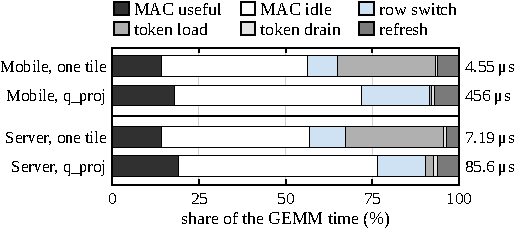
\includegraphics[width=\columnwidth]{figs/fig_breakdown.pdf}
  \caption{Stock AiM's GEMM time by component.}
  \label{fig:breakdown}
\end{figure}

% P:mot-nonmac-classes
\paragraph{Non-MAC commands}
Non-MAC commands (Section~\ref{sec:bg:pim}) stall every PU: no PU starts a MAC while they run. The four non-MAC
segments of Fig.~\ref{fig:breakdown}, row switch, token load, token drain and refresh, form three classes. The
\emph{row-switch commands}, the two TMODs, the PREA and ACT16 pair of each row opened and the WRMAC16, cost the
\emph{row-switch overhead} \trow once per row sweep. The \emph{token load/drain commands}, each token's share of WRGB
(token load) and its RDMAC16 (token drain), cost \ttok once per token. Refresh, the third class, blocks every command
for $t_\mathrm{RFCab}$ once per $t_\mathrm{REFI}$ (Table~\ref{tab:params}). With one token per stock row sweep, a GEMM
pays a row's row-switch commands $M$ times, where a GEMV pays them once.

% P:mot-rowswitch-cost
Row-switch commands are the largest class of non-MAC commands. In Fig.~\ref{fig:breakdown} the row-switch segment
takes 19.5\,\% of q\_proj's time on the mobile platform, more than the useful beats' 18.0\,\%, and 13.8\,\% on the edge
server. The two TMODs (8.1\,\%) and the ACT16 pair (8.5\,\%, timed by a simulator preset) take most of the mobile row
switch. The other two classes take less of q\_proj's time. Token load and token drain take at most 2.4\,\% and
1.0\,\%, because one GB fill serves all 64 row sweeps (mobile) or 16 (edge server) over its $K$ chunk, and refresh
takes 7.1\,\% on the mobile platform and 6.2\,\% on the edge server. On the edge server, the non-MAC commands together
take 23.4\,\%, more than the useful beats' 19.1\,\%.

% P:mot-sweep-factor
We define the share of the GEMM time that the MAC slots get as the \emph{sweep factor} \fMAC. For a row sweep of
$c$ MAC slots that serves $A$ tokens, the row-switch overhead, the token load/drain and refresh set \fMAC:
\begin{equation}
  \fMAC = \frac{(1 - \rho)\, c\, \tslot}{c\, \tslot + \trow + A\, \ttok}, \label{eq:fmac}
\end{equation}
where $\rho$ is the share of time that refresh takes. Fitted on stock AiM at $M = 1$ on the mobile platform, \trow
is 87.73\,ns, \ttok is 4.26\,ns and $\rho$ is 0.070, so stock AiM's MAC slots fill $\fMAC = 0.717$ of a decoder layer's
time.

% P:mot-idle-beats
\paragraph{Idle beats}
An idle beat is a CK cycle in which a PU has nothing to compute. A column period holds $D = 4$ such cycles, or beats
(Section~\ref{sec:bg:pim}), and a beat is useful when it computes a token's MAC. Stock AiM's MAC slot serves one token,
so one beat of each column period is useful and three are idle (Fig.~\ref{fig:dram_pim}b). The \emph{slot factor},
the useful share of a MAC slot, is $\UMAC = A \times b \times \tck / \tslot$, where $b$ is the number of beats per
token: $b = 1$ on the mobile platform, and $b = 2$ on the edge server, where each MAC command feeds a PU from its two
banks. Stock AiM's \UMAC is therefore 1/4. The idle segment is the largest of every bar in Fig.~\ref{fig:breakdown},
53.9\,\% of q\_proj's time on the mobile platform and 57.4\,\% on the edge server, three times the useful beats.

% P:mot-idle-cause
Idle beats arise because the column command, not the PU, paces every stock MAC: a MAC starts only when a column command
delivers its weights. HBM-PIM~\cite{hbmpim} executes one instruction per column command, and AiM~\cite{aimjssc} clocks
its PU at its interface's $t_\mathrm{CCD}$. Each column command reads one column, and DRAM timing lets the next column
command follow only after \tccds{} or \tccdl. Command pacing suits a GEMV, the target of these
PUs~\cite{aimjssc,p3llm}: in a GEMV each weight column meets one input vector, so one beat per column is enough.
Replacing stock AiM's PU, which runs one beat per column period, with a PU four times faster, clocked at CK, leaves
every stock GEMM at the same number of cycles.

% P:mot-utilization
The two losses multiply. The useful-MAC utilization $U$ is the MAC-useful share of each bar in
Fig.~\ref{fig:breakdown} and equals $W \times \tck / T_\mathrm{GEMM}$, where $W$ is the number of useful beats per PU
and $T_\mathrm{GEMM}$ is the GEMM time; $U$ thus measures a design against a PU that runs one useful beat per CK cycle. $U$ is the product
of the slot factor and the sweep factor, $U = \UMAC \times \fMAC$.
% useful-MAC table (cited first in III-B's closing paragraph): defined inside that paragraph so that it lands at the top
% of the column that cites it; generated by scripts/make_tables.py (simulated values, evaluation/dac_2x2 Sec. 2h)
\begin{table}[t]
  \caption{Useful-MAC utilization on the mobile platform.}
  \label{tab:umac}
  \centering
  \footnotesize
  \setlength{\tabcolsep}{3pt}
  % generated by scripts/make_tables.py from evaluation/dac_2x2/figures/tab_umac_paper.csv (umacp ids, simulated columns, M = 8); do not edit
\begin{tabular}{@{}lcccccc@{}}
\toprule
Design & $A$ & \tslot & \UMAC & \fMAC & $U$ & Non-MAC \\
 & & ns & & & & ns/token \\
\midrule
Stock AiM & 1 & 5 & 0.25 & 0.717 & 0.179 & 123.39 \\
P3-LLM-style & 2 & 5 & 0.50 & 0.709 & 0.355 & 63.94 \\
LP-Spec-style (4 ALUs) & 4 & 5 & 1.00 & 0.694 & 0.694 & 34.41 \\
\textbf{CoDe} ($V = 8$) & 8 & 10 & 1.00 & 0.779 & 0.779 & 22.15 \\
\bottomrule
\end{tabular}

\end{table}
Stock AiM's $U$ is $1/4 \times 0.717 = 0.179$ on the mobile platform (Table~\ref{tab:umac}) and 0.193 on the edge
server. Section~\ref{sec:bg:walls} examines how prior PIM designs answer each root cause.

\subsection{GEMM Support in Prior PIM}
\label{sec:bg:walls}

% P:mot-prior-families
Prior PIM designs fill the idle beats in two families, with more multipliers or with more commands
(Fig.~\ref{fig:timeline}). Fig.~\ref{fig:timeline} follows one weight column through eight tokens in stock AiM and in
one design of each family, LP-Spec~\cite{lpspec} for more multipliers and P3-LLM~\cite{p3llm} for more commands; the
next paragraphs take the two families in turn.

% P:mot-wider-pu
\paragraph{Wider-PU family}
Wider-PU designs trade area for MAC throughput: they fill the idle beats with more multipliers per PU.
LP-Spec~\cite{lpspec} builds its matrix unit from four 32-wide INT8 ALUs, clocks the ALUs at one MAC step per column
period, and shares one unit between two banks; we model one such unit per bank (Table~\ref{tab:params}). One column
command feeds the four ALUs with four tokens, one MAC step each. Fig.~\ref{fig:timeline} counts one bank's time in
column periods $T$ of $D = 4$ beats: where stock AiM spends 8 column periods, 8 commands and 8 reads on the 8 tokens,
the four ALUs need 2 of each, on four times the stock multipliers. The 4$\times$ ceiling moves the crossover of this
per-bank design with the host to $M = 20$--24 on the mobile platform (Fig.~\ref{fig:roofline}a).
PAPI~\cite{papi} places four processing units in each bank, and StepStone~\cite{stepstone} places SIMD units at the
bank groups or beside the devices of a memory module. Duplex~\cite{duplex} and H$^2$-LLM~\cite{h2llm} build their
multipliers on a logic die under the DRAM, and MoNDE~\cite{monde} builds them into a memory-side controller. We take
LP-Spec~\cite{lpspec} as the representative of the wider-PU family and model it as an \textbf{LP-Spec-style} design,
the rival on the mobile platform (Section~\ref{sec:eval:phone}). LP-Spec-style's slot serves four tokens, so
LP-Spec-style reaches $\UMAC = 1$ (Table~\ref{tab:umac}) only by quadrupling the multipliers: per multiplier its $U$
is 0.173--0.174 on the mobile platform and 0.185 on the edge server, below stock AiM's.

% timeline figure (cited first in III-C's opener; defined after mot-wider-pu so that it lands on the next page, not
% under Table I): column-width schematic; generated by scripts/make_fig_timeline.py
\begin{figure}[t]
  \centering
  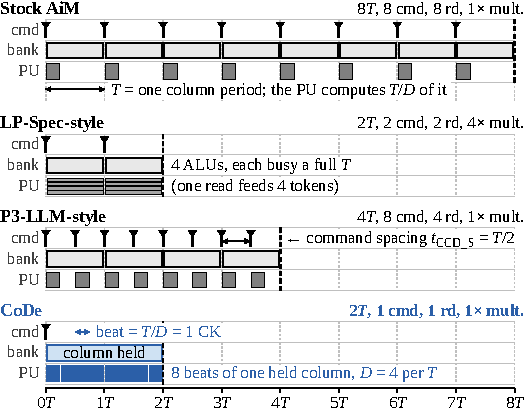
\includegraphics[width=\columnwidth]{figs/fig_timeline.pdf}
  \caption{One weight column of one bank in four designs; lanes show DRAM commands (cmd), column reads (bank) and MAC
  beats (PU).}
  \label{fig:timeline}
\end{figure}

% P:mot-logic-cost
\paragraph{Cost of logic in a DRAM die}
Logic in a DRAM die costs area: UPMEM~\cite{devaux} reports that a DRAM process builds logic 10$\times$ less dense
than an ASIC process and routes the logic in three metal layers instead of ten or more. In GDDR6-AiM~\cite{aimjssc} silicon, one PU occupies
0.19\,mm$^2$. Samsung's HBM-PIM~\cite{hbmpim} halves its DRAM sub-arrays to make room for its PUs and so gives up 50\,\% of
the die's memory capacity. By LP-Spec's~\cite{lpspec} own estimate its compute units and buffers take
16.92\,\% of a 16\,Gb LPDDR5 die, against 20--25\,\% of the chip for all of AiM's~\cite{aimjssc} compute circuits.
Four times the multipliers per bank therefore cost capacity, and per unit of logic area the wider-PU family keeps
only part of its 4$\times$ ceiling: LP-Spec-style's ceiling per logic mm$^2$ is 314\,GOPS on the mobile platform and
697 on the edge server, against stock AiM's 216 and 492.

% P:mot-faster-pu
\paragraph{Faster-PU family}
Faster-PU designs speed up the PU but still start every MAC with a command, so DRAM command timing, not the PU clock,
caps them at two beats per column read. P3-LLM~\cite{p3llm} keeps the weight of a column read latched in its PU,
issues one further command per token and clocks its PU at one beat per HBM2 \tccds{} (Table~\ref{tab:params}). Each
MAC thus still waits for its own command, as in stock AiM and LP-Spec-style (Fig.~\ref{fig:timeline}). Commands issue
only every \tccds, ``typically a half of \tccdl{}''~\cite{p3llm}, while the all-bank column runs at
\tccdl~\cite{hbmpim}, so at most two tokens share a read: the 8 tokens take 4 column periods, 8 commands and 4 reads.
On every memory family whose \tccdl{} is twice \tccds{}, the faster-PU family's \UMAC therefore stops at 1/2 however
fast its PU runs. The 2$\times$ ceiling moves the crossover of this design with the host to $M = 4$--6 on the edge
server (Fig.~\ref{fig:roofline}b). P3-LLM~\cite{p3llm} is the only design that applies a faster PU to $M > 1$, so we
take P3-LLM as the representative of the faster-PU family and model it as a \textbf{P3-LLM-style} design, the rival on
the edge server (Section~\ref{sec:eval:server}). With the stock multiplier count, P3-LLM-style's ceiling per logic
mm$^2$, 390\,GOPS on the mobile platform and 830 on the edge server, lies above LP-Spec-style's.

% P:mot-other-pim
The remaining LLM PIM designs fall outside the wider-PU and faster-PU families. GEMV-only designs serve one input
vector per weight read~\cite{newton,cent,pimgpt}, lookup-table designs replace multiplications with table
lookups~\cite{localut,pimpal,pimdl}, and scheduling and dataflow designs reorganize the work around the
PU~\cite{pimba,paise,splitsync,dots,pimphony}. Three designs, the closest prior art, run several MAC beats per column
read, yet each design holds one input vector ($M = 1$): SAL-PIM~\cite{salpim} clocks its MAC units at twice the column
rate, the Precision-Flexible PU~\cite{pfpu} runs four phases per column interval on packed low-bit operands, and
CD-PIM~\cite{cdpim} runs two compute units per bank at twice the internal clock. CD-PIM~\cite{cdpim} leaves the GEMM to
the host processor, and the extra beats of all three designs work on the same vector. Across the two families and
these three designs, a column read feeds several tokens only through added multipliers or added commands, and a row
sweep serves only the tokens of one MAC slot.

\subsection{The Opportunity: DRAM Timing Bounds Access, Not MACs}
\label{sec:bg:depth}

% P:mot-depth
DRAM timing bounds how often a column is read, not how many MACs may consume it. The PU takes its operands from the I/O sense amplifiers at the bank's I/O
boundary~\cite{hbmpim}, so a column the PU has latched stays usable after its command: P3-LLM~\cite{p3llm} reuses a
latched column for two tokens at unchanged cell-access and column-decoder power, the majority of PIM power. The column
period thus sets how often weights arrive at a PU, and the PU clock sets how often the PU computes on them, so a PU
clocked at CK can spend all $D$ beats of a column period on one latched column, as long as its MACs do not wait for
per-token commands.

% P:mot-pu-clock-precedent
A PU clocked at CK has precedent in DRAM silicon and in a PIM design for HBM2. HBM2's DRAM core runs at a quarter of
the 1.0--1.2\,GHz bus clock, and Samsung's HBM-PIM~\cite{hbmpim} sets its FP16 PU to the core frequency,
250--300\,MHz, in a 20\,nm DRAM process. Logic in later DRAM processes runs faster: UPMEM's processor~\cite{devaux}
is designed to execute 32-bit integer instructions at 500\,MHz in a 2x-nm DRAM process, a deployed UPMEM system
runs the processor at 350\,MHz~\cite{prim}, and GDDR6-AiM~\cite{aimjssc} runs BF16
multipliers and adder trees at 1\,GHz in a 1y-nm DRAM process. The 1y-nm process also builds HBM: Samsung's
HBM2E~\cite{flashbolt} stacks eight 1y-nm DRAM dies. The Precision-Flexible PU~\cite{pfpu} clocks an HBM-PIM-style
PU at CK on HBM2 and splits each 4-\tck column interval into four phases. DRAM periphery has gained logic-process
features: Samsung, SK hynix and Micron build periphery transistors with high-k metal gates~\cite{tiroadmap}, and
1a-nm dies route in five to six metal layers~\cite{tid1a16,tid1a24}.

% P:mot-two-levers
A PU at CK thus fits in a DRAM die, and the wider-PU family shows how much logic area a PIM die already gives to
filling idle beats. We therefore keep the stock multipliers, run them at CK within that area, and answer each root
cause of Section~\ref{sec:bg:cmd} with one lever. \emph{Row reuse} (Section~\ref{sec:design:reuse}) lets the $V$
tokens of a tile share one row sweep and pay its row-switch commands once, and answers the non-MAC commands by cutting
their time per token. \emph{Beat filling} (Section~\ref{sec:design:beat}) uses all $D$ beats of a column period
(Fig.~\ref{fig:dram_pim}b) without adding multipliers and answers the idle beats.
